\section{Evaluation}\label{eval}
We evaluate the implemented type inference engine on a number of benchmarks. First, the performance of \core is compared against the subtyping based system. Subtyping collects all constraints throughout the type inference, while \core solves each constraint immediately. I made the hypothesis that \core should be faster than subtyping. 

Secondly, \core represents types in a smaller and cleaner format compared to subtyping (due to not having any explicit constraints anymore). Several programs are tested in both systems in order to manually compare them. 

All benchmarks were run on a MacBook Pro with an 2.5 GHz Intel Core I7 processor and 16 GB 1600 MHz DDR3 RAM running Mac OS 10.13.4.

\subsection{Performance Comparison}

Our first evaluation, in figure~\ref{fig:loops}, considers five different testing programs:
\todo{explanation interp, loop, parser, queens, range}
\begin{enumerate}
\item \texttt{Interp}, 
\item \texttt{Loop}, 
\item \texttt{Parser}, 
\item \texttt{Queens}, 
\item \texttt{Range},
\end{enumerate}

These programs are compiled with three different type systems:
\begin{enumerate}
\item Subtyping type system, the "old" type system from the Eff programming language. 
\item \core, the system proposed in this thesis, based upon extending algebraic subtyping with algebraic effects and handlers.
\item Untyped system, the Eff programming language without type inference.
\end{enumerate}

The different systems are all implemented in the \eff programming language. Thus, they share many different aspects of the implementation, including parsing, lexing and the runtime. The Untyped system does not compute any types, while the other two systems do use type inference engines. 

Figure~\ref{fig:test} shows the time relative to the Untyped version for running each of
the programs for 10,000 iterations. Overall, the performance of \core is superior to the performance of standard subtyping. There is an exception for the \texttt{Queens} program. The implementation of \core is very slow compared to the other implementations. This is a very strange anomaly as it was completely unexpected. I hypothezise that the lack of a simplification algorithm causes the huge slowdown. Because the simplification of the types never occurs, the types keep growing in size. Due to this, any constraints that are introduced during type inference are also very large in size, which causes the slowdown. 

\todo{give and explain the results}

\begin{figure}[H]
\centering
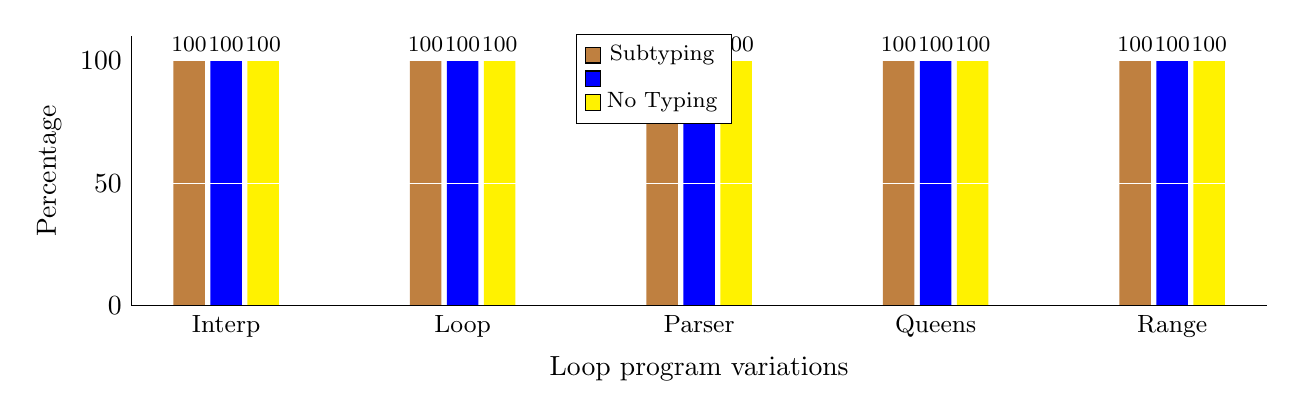
\begin{tikzpicture}
    \centering
    \begin{axis}[
        ybar, axis on top,
        height=5cm, width=16cm,
        ymajorgrids, tick align=inside,
        bar width=0.4cm,
        major grid style={draw=white},
        enlarge y limits={value=.1,upper},
        ymin=0, ymax=100,
        axis x line*=bottom,
        axis y line*=left,
        y axis line style={opacity=1},
        tickwidth=0pt,
        xtick = data,
        x tick label style={font=\small,text width=1.4cm,align=center},
            enlarge x limits=true,
        legend image code/.code={%
        \draw[#1] (0cm,-0.1cm) rectangle (0.2cm,0.1cm);
    },
            legend style={
            at={(0.46,1.01)},
            anchor=north,
            % legend columns=-1,
            % /tikz/every even column/.append style={column sep=0.4cm},
            font = \footnotesize
        },
        ylabel={Percentage},
        xlabel={Loop program variations},
            symbolic x coords={
            Interp,
            Loop,
            Parser,
            Queens,
            Range,
            },
            nodes near coords={
            \footnotesize \pgfmathprintnumber{\pgfplotspointmeta}
        }
    ]
    \addplot [draw=none,fill=brown] coordinates {
        (Interp,100)
        (Loop,100)
        (Parser,100)
        (Queens,100)
        (Range,100)
    };

    \addplot [draw=none,fill=blue] coordinates {
        (Interp,100)
        (Loop,100)
        (Parser,100)
        (Queens,100)
        (Range,100)
    };

    \addplot [draw=none,fill=yellow] coordinates {
        (Interp,100)
        (Loop,100)
        (Parser,100)
        (Queens,100)
        (Range,100)
    };
    
    \legend{Subtyping, \core, No Typing}
    \end{axis}
    \end{tikzpicture}
\caption{Relative run-times of testing programs}
\label{fig:test}
\end{figure}
    
\subsection{Type Inference Comparison}

The main contribution of this thesis is to extend the algebraic subtyping algorithm with algebraic effects and handlers. The goal is to be able to infer types which are shorter, simpler and more human-readable than types inferred by standard subtyping systems. In this evaluation, several small programs were made and its types inferred by the subtyping and the algebraic subtyping system in order to compare both types. 

Considering that the implementation does not yet support the simplification of types, the results are inaccurate. In order to provide a proper evaluation, the types have been manually simplified using the simplification algorithm. All three types are given in order to the current state of the implementation and to be able to evaluate the algebraic subtyping system.


\todo{give the evaluation results}

\begin{figure}[H]
\begin{center}
\begin{framed}
\begin{minipage}[t]{0.95\columnwidth}
    \begin{mathpar}
    \inferrule[Interp]{}{
        \ctxp \prinent x \T [x : \alpha]\alpha
    }

    \inferrule[Loop]{}{
        \ctxp \prinent x \T [x : \alpha]\alpha
    }

    \inferrule[Parser]{}{
        \ctxp \prinent x \T [x : \alpha]\alpha
    }

    \inferrule[Queens]{}{
        \ctxp \prinent x \T [x : \alpha]\alpha
    }

    \inferrule[Range]{}{
        \ctxp \prinent x \T [x : \alpha]\alpha
    }
\end{mathpar}
\end{minipage}
\end{framed}
\end{center}
\caption{Produced types for Subtyping}\label{fig:inferred:sub}
\end{figure}

\begin{figure}[H]
\begin{center}
\begin{framed}
\begin{minipage}[t]{0.95\columnwidth}
    \begin{mathpar}
    \inferrule[Interp]{}{
        \ctxp \prinent x \T [x : \alpha]\alpha
    }

    \inferrule[Loop]{}{
        \ctxp \prinent x \T [x : \alpha]\alpha
    }

    \inferrule[Parser]{}{
        \ctxp \prinent x \T [x : \alpha]\alpha
    }

    \inferrule[Queens]{}{
        \ctxp \prinent x \T [x : \alpha]\alpha
    }

    \inferrule[Range]{}{
        \ctxp \prinent x \T [x : \alpha]\alpha
    }
\end{mathpar}
\end{minipage}
\end{framed}
\end{center}
\caption{Produced types for \core}\label{fig:inferred:core}
\end{figure}

\begin{figure}[H]
\begin{center}
\begin{framed}
\begin{minipage}[t]{0.95\columnwidth}
    \begin{mathpar}
    \inferrule[Interp]{}{
        \ctxp \prinent x \T [x : \alpha]\alpha
    }

    \inferrule[Loop]{}{
        \ctxp \prinent x \T [x : \alpha]\alpha
    }

    \inferrule[Parser]{}{
        \ctxp \prinent x \T [x : \alpha]\alpha
    }

    \inferrule[Queens]{}{
        \ctxp \prinent x \T [x : \alpha]\alpha
    }

    \inferrule[Range]{}{
        \ctxp \prinent x \T [x : \alpha]\alpha
    }
\end{mathpar}
\end{minipage}
\end{framed}
\end{center}
\caption{Produced types for Algebraic Subtyping}\label{fig:inferred:manual}
\end{figure}